\documentclass[a4paper]{article}
\usepackage{xeCJK}
\setmainfont{DejaVu Serif}
\setCJKmainfont{WenQuanYi Micro Hei}

%opening
\title{Linear Regression}
\author{onerhao}

\usepackage{amssymb,amsmath,bm,amsthm}
\usepackage{textcomp}
\usepackage{longtable}
\usepackage{algorithm2e}
\usepackage{tocbibind}
\usepackage[toc]{multitoc}
\usepackage{mathptmx}        % selects Times Roman as basic font
\usepackage{helvet}          % selects Helvetica as sans-serif font
\usepackage{courier}         % selects Courier as typewriter font
%\usepackage{type1cm}        % activate if the above 3 fonts are 
% not available on your system

\usepackage{makeidx}         % allows index generation
\usepackage{graphicx}        % standard LaTeX graphics tool
% when including figure files
\usepackage[justification=centering]{caption}
\usepackage{subfig}
\usepackage{multicol}        % used for the two-column index
\usepackage{multirow}
\usepackage[bottom]{footmisc}% places footnotes at page bottom
\usepackage[bookmarksnumbered=true,
bookmarksopen=true,
colorlinks=true,
linkcolor=blue,
anchorcolor=blue,
citecolor=blue
]{hyperref}



% 调整页面
\usepackage[scale=0.75]{geometry}


\begin{document}

	

\maketitle

\begin{abstract}

\end{abstract}

\section{介绍}
线性回归通常是被人为是最简单的机器学习模型。但是却有着非常广泛的应用,其表现形式也是很多其他模型的基础.统计学线性回归就是我们大家几乎都用过的模型,用最小二乘法来拟合直线,得到直线的两个参数.在事迹应用中更多的是高维空间.线性回归其实还有这另外一种形式,就是贝叶斯线性回归。这种模型假定模型参数有一个先验概率,并且用最大后验概率来求解。从最终解的行驶上很容易看出它和高斯过程的关系、以及核函数的引入。


\section{模型}

\begin{equation}
p(y|\vec{x},\vec{\theta})=\mathcal{N}(y|\vec{w}^T\vec{x}, \sigma^2)
\end{equation}
这里$\vec{w}$ 和 $\vec{x}$ 是extended vectors,满足 $\vec{x}=(1,x)$, $\vec{w}=(b,w)$.
线性回归可以用于拟合非线性关系,只需要把$\vec{x}$替换成一些非线性的作用于输入上的basis function $\phi(\vec{x})$ \begin{equation}
p(y|\vec{x},\vec{\theta})=\mathcal{N}(y|\vec{w}^T\phi(\vec{x}), \sigma^2)
\end{equation}
这个过程被称为\textbf{basis function expansion}。注意,这个模型仍然被称为线性线性,因为参数$\vec{w}$是线性的。一个简单的例子是多项式拟合,其模型如下:
\begin{equation}
\phi(x)=(1, x, \cdots, x^d)
\end{equation}


\section{最大似然然估计}
对于一个统计模型,一个常用的估计参数的方法就是最大似然估计。在先前假定了这个回归模型的目标值$t$服从高斯分布,由高斯分布的指数形式,求取对数后也就是我们很熟悉的最小二乘法的优化问题。
\begin{equation}
\vec{\hat{\theta}}=\arg\max_\theta{logp(D|\vec{\theta})}
\end{equation}
对于所有数据集,似然函数就是
\begin{align}\label{eqn:linear regression likelihood}
p(\vec{t}|\vec{X},\vec{w},\beta) =
\prod_{n=1}^{N}\mathcal{N}(t_n|\vec{w}^T\phi(\vec{x_n}),\beta^{-1})
\end{align}
参数就是使得似然函数最大的值。
假设所有训练数据都是独立同分布的\textbf{independently and identically distributed(IID)},我们可以把对数似然函数\textbf{log-likelihood} function写成:
\begin{equation}
\ell(\vec{\theta}) \triangleq \log p(\mathcal{D}|\vec{\theta})
\end{equation}
最大化似然函数等价于最小化\textbf{negative log likelihood}:
\begin{equation}
\text{NLL}(\vec{\theta}) \triangleq -\ell(\vec{\theta})=-\log p(\mathcal{D}|\vec{\theta})
\end{equation}
因为很多软件是为求最小值设计的,所以有时候负对数似然函数可能更加方便。下面我们看看最大似然估计的解法.
\begin{align}
\ell(\vec{\theta})& =\sum\limits_{i=1}^N \log\left[\dfrac{1}{\sqrt{2\pi}\sigma}\exp\left(-\dfrac{1}{2\sigma^2}(y_i-\vec{w}^T\vec{x}_i)^2\right)\right] \\
& =-\dfrac{1}{2\sigma^2}\text{RSS}(\vec{w})-\dfrac{\vec{w}}{2}\log(2\pi\sigma^2)
\end{align}

我们可以把\textbf{log-likelihood} (对数似然函数) 重写成:
\begin{equation}
\ell(\vec{\theta}) \triangleq \log p(\mathcal{D}|\vec{\theta})
\end{equation}
替换高斯函数的形式,我们得到:
\begin{align}
\ell(\vec{\theta}) &= \log p(\vec{T}|\vec{w},\beta) \\
&=\sum_{n=1}^{N}\log \mathcal{N}(t_n|\vec{w}^T\phi(\vec{x_n}),\beta^{-1}) \\
&=\sum\limits_{i=1}^N \log\left[\dfrac{1}{\sqrt{2\pi}\sigma}\exp\left(-\dfrac{1}{2\sigma^2}(y_i-\vec{w}^T\vec{x}_i)^2\right)\right] \\
&=\dfrac{N}{2}\log \beta-\dfrac{N}{2}\log (2\pi)-\beta E_D(\vec{w}) \\
&=-\dfrac{1}{2\sigma^2}\text{RSS}(\vec{w})-\dfrac{\vec{w}}{2}\log(2\pi\sigma^2)
\end{align}
这里平方和就是
\begin{equation}
E_D(\vec{w}) =
\dfrac{1}{2}\sum_{n=1}^{N}\{t_n-\vec{w}^T\phi(\vec{x_n}) \}^2
\end{equation}
RSS 表示 \textbf{residual sum of squares}等于
\begin{equation}
\text{RSS}(\vec{w}) \triangleq \sum\limits_{i=1}^N (t_i-\vec{w}^T\vec{x}_i)^2
\end{equation}
RSS 也可以写成residual errors 的$\ell_2$ \textbf{正则形式}:
\begin{equation}
RSS(\vec{w}) = \parallel\epsilon\parallel_2^2 = \sum_{i=1}^{N}\epsilon_i^2
\end{equation}
这里 $\epsilon_i = (t_i - \vec{w}^T\vec{x_i})$.
有两种方式求解。
\subsection{MLE推导}
这里我们会看到对高斯分布的最大似然求解最终形式就是最小二乘法的求解过程。
\begin{equation}
\nabla\log p(\vec{t}|\vec{w},\beta)
=\sum_{n=1}^{N}\{t_n-\vec{w}^T\phi(\vec{x_n}) \}\phi(\vec{x_n})^T
\end{equation}

关于 $\vec{w}$ 的常数可以忽略掉
\begin{equation}
\text{NLL}(\vec{w}) = \dfrac{1}{2}\sum\limits_{i=1}^N (y_i-\vec{w}^T\vec{\phi}_i)^2
\end{equation}

定义 $\vec{y}=(t_1,t_2,\cdots,t_N)$, $\vec{\Phi}=\left(\begin{array}{c}\vec{\phi}_1^T \\ \vec{\phi}_2^T \\ \vdots \\ \vec{\phi}_N^T\end{array}\right)$, 我们可以将目标函数写成一种更加合适的形式:
\begin{align}
\text{NLL}(\vec{w}) &= \dfrac{1}{2}(\vec{t}-\vec{\Phi}\vec{w})^T(\vec{t}-\vec{\Phi}\vec{w})\\
&= \dfrac{1}{2} [\vec{w^T} (\vec{\Phi}^T\vec{\Phi})\vec{w} - \vec{t}^T\vec{\Phi}\vec{w}- \vec{w}^T\vec{x}^T\vec{t}  +\vec{t}^T\vec{t}]			\\
\Rightarrow
\dfrac{\partial}{\partial \vec{w}}\text{NLL} &= \dfrac{1}{2} \vec{w^T} (\vec{\Phi}^T\vec{\Phi})\vec{w} -\vec{w}^T(\vec{\Phi}^T\vec{t}) 
\end{align}
这里
$\begin{cases}
\vec{\Phi} = \begin{bmatrix}
&\vec{\Phi_1^T} \\
&\vec{\Phi_2^T} \\
& ... \\
&\vec{\Phi_n^T}
\end{bmatrix} \\	
\vec{\Phi^T}\vec{\Phi} =
\begin{bmatrix}
\vec{\Phi_1} & \vec{\Phi_2} & ...&\vec{\Phi_n}
\end{bmatrix} 
\cdot
\begin{bmatrix}
&\vec{\Phi_1^T} \\
&\vec{\Phi_2^T} \\
& ... \\
&\vec{\Phi_N^T}
\end{bmatrix}  = \sum\limits_{i=1}^{N}\vec{\phi_i}\vec{\phi_i^T} = \textbf{平方和矩阵} \\
\end{cases}$

需要注意的是 $\vec{\Phi}$是一个$N\times M$ 矩阵,被称为\textbf{design matrix},它的元素是 $\Phi_{nj}=\phi_j(\vec{x_n})$ so that
\begin{equation}
\vec{\Phi}=
\begin{bmatrix}
\phi_0(\vec{x_1}) &	\phi_1(\vec{x_1}) &...&\phi_{M-1}(\vec{x_1}) \\
\phi_0(\vec{x_2}) & \phi_1(\vec{x_2}) &...&\phi_{M-1}(\vec{x_2}) \\
\vdots &\vdots &\vdots&\vdots \\
\phi_0(\vec{x_N})& \phi_1(\vec{x_{N}})& \cdot &\phi_{M-1}(\vec{x_N})\\
\end{bmatrix}
\end{equation}

当$\mathcal{D}$ 比较小(比如, $N < 1000$),我们可以直接直接计算$\vec{w}$
\begin{equation}
\vec{w}_{ML}=\hat{\vec{w}}_{\mathrm{OLS}}=(\vec{\Phi}^T\vec{\Phi})^{-1}\vec{\Phi}^T\vec{t}
\end{equation}
这个解$\hat{\vec{w}}_{\mathrm{OLS}}$ 被称为\textbf{ordinary least squares} or \textbf{OLS} or \textbf{normal equation},也就是通解.

简单的证明过程如下:
\begin{proof}
	利用$\mathbf{向量-向量}$ 微分,如果 $\mathbf{A}$ 不是 $\vec{x}$ 的函数,那么
	\begin{equation}
	\dfrac{\partial\vec{X}^TA\vec{X}}{\partial\vec{X}} = \vec{X}^T(\mathbf{A}+\mathbf{A}^T) = (\mathbf{A}+\mathbf{A}^T)\vec{X}
	\end{equation}
\end{proof}
然后,推导 $\dfrac{\partial NLL}{\partial \vec{w}}$
\begin{eqnarray}
g(\vec{w}) &= \dfrac{\partial NLL}{\partial\vec{w}} \\
&=\vec{\Phi}^T\vec{\Phi}\vec{w} - \vec{\Phi}^T\vec{y}			
\end{eqnarray}
让导数为零
\begin{equation}
\vec{w} = (\vec{X}^T\vec{X})^{-1}\vec{x}^T\vec{y}
\end{equation}

\subsection{几何解释}

\ref{fig:graphical-interpretation-of-OLS}.
\begin{figure}[hbtp]
	\centering
	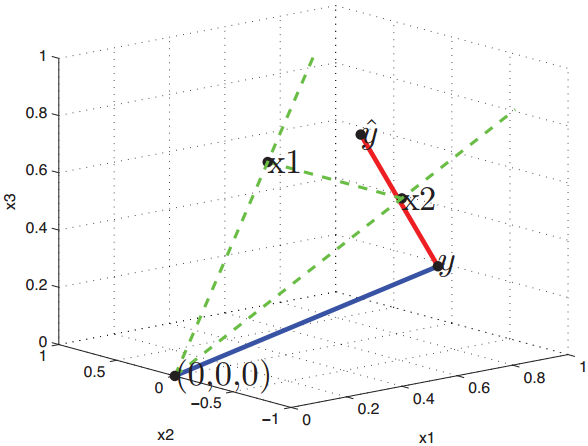
\includegraphics[scale=.50]{graphical-interpretation-of-OLS.png}
	\caption{Graphical interpretation of least squares for $N=3$ examples and $D=2$ features. $\tilde{\vec{x}}_1$ and $\tilde{\vec{x}}_2$˜ are vectors in $\mathbb{R}^3$; together they define a 2D plane. $\vec{y}$ is also a vector in $\mathbb{R}^3$ but does not lie on this 2D plane. The orthogonal projection of $\vec{y}$ onto this plane is denoted $\hat{\vec{y}}$. The red line from $\vec{y}$ to $\hat{\vec{y}}$ is the residual, whose norm we want to minimize. For visual clarity, all vectors have been converted to unit norm.}
	\label{fig:graphical-interpretation-of-OLS} 
\end{figure}
将输入数据集矩阵写成行向量形式,
\begin{eqnarray}
\vec{X} = \begin{bmatrix}
\vec{x_1}^T &\\
\vec{x_2}^T &\\
...        &\\
\vec{x_N}^T
\end{bmatrix} 
= \begin{bmatrix}
\vec{\tilde{x_1}} & \vec{\tilde{x_1}} & ... &\vec{\tilde{x_D}}
\end{bmatrix}\\
\vec{y} = \begin{bmatrix}
t_1 \\
t_2 \\
... \\
t_n
\end{bmatrix} 
\end{eqnarray}
我们的求解目标就是找到一个$\hat{\vec{t}} \in \mathbb{R}^N$ ,在$\vec{X}$的列线性空间并且尽可能的接近预测值$\vec{t}$,也就是寻找
\begin{eqnarray}
\hat{\vec{t}} \in span(\vec{X}) \\
\Rightarrow \hat{\vec{t}} = \vec{X}\vec{w} = w_1\vec{\tilde{x_1}}+\cdot\cdot\cdot+w_D\vec{\tilde{x_D}} \\
\vec{\hat{t}}=\arg\min\limits_{\hat{\vec{t}} \in \text{span} (\{\vec{\tilde{x_1}},...,\vec{\tilde{x_D}}\})}
\end{eqnarray}

为了最小化正则误差, $\vec{y}-\hat{\vec{y}}$, 残留误差向量与 $\vec{X}$中每一列都垂直 $\tilde{\vec{x}}_j(\vec{y}-\hat{\vec{y}})=0$ for $j=1:D$.那么
\begin{equation}\begin{split}
\tilde{\vec{x}}_j(\vec{y}-\hat{\vec{y}})=0 & \Rightarrow \vec{X}^T(\vec{y}-\vec{X}\vec{w})=0 \\
& \Rightarrow \vec{w}=(\vec{X}^T\vec{X})^{-1}\vec{X}^T\vec{y}
\end{split}\end{equation}


\subsection{在线学习}
Batch学习方式,比如最大似然解,涉及到在每一轮对整个数据集进行处理,这对大数据来讲就非常的消耗资源。如果这个数据集的确足够大,那么我们可以使用\textbf{在线学习(online-learning)},在每轮中处理一个数据.当数据集$\mathcal{D}$足够大时,我们适用\textbf{随机梯度下降-stochastic gradient descent(SGD)}来求解最值问题.
\begin{align}
E &=\sum_{n}E_n \\
\vec{w}^{\tau+1} &= \vec{w}^{\tau}-\eta\nabla E_n
\end{align}
这里 $\tau$表示迭代次数,$\eta$学习速率参数.这里,在我们的平方和误差公式中
\begin{equation}
\vec{w}^{\tau+1} = \vec{w}^{\tau}-\eta(t_n-\vec{w}^{(\tau)T}\phi_n)\phi_n
\end{equation}
这里$\phi_n=\phi(\vec{x_n})$.具体演算如下:
\begin{align}
\because \dfrac{\partial}{\partial w_i}\text{NLL}(\vec{w})=& \sum\limits_{i=1}^N (\vec{w}^T\vec{x}_i-y_i)x_{ij} \\
\therefore w_j=& w_j - \alpha\dfrac{\partial}{\partial w_j}\text{NLL}(\vec{w}) \nonumber \\
=& w_j - \sum\limits_{i=1}^N \alpha(\vec{w}^T\vec{x}_i-y_i)x_{ij} \\
\therefore \vec{w}=& \vec{w}-\alpha(\vec{w}^T\vec{x}_i-y_i)\vec{x}
\end{align}

\section{岭回归(MAP)}
岭回归就是加上了正则化项来控制模型复杂度来避免过拟合的。而贝叶斯线性回归不仅可以避免过拟合,还可以进行online-learning。所以这里就不细讲岭回归了。

\section{Bias-Variance分解}
这个可以参看我的前一篇文章。

\section{贝叶斯线性回归}
保留数据来用于决定模型复杂度是一种防止过拟合的方法,但是这在计算上却要求很多的资源,因为我们需要重复的训练、验证。并且这还可能浪费一部分宝贵的数据。所以我们需要贝叶斯线性回归,这个模型可以自动决定模型复杂度,并且利用每一个数据进行训练。
\subsection{参数分布}
首先我们需要估计模型的参数的先验分布.这个似然函数$p(\vec{t}|\vec{w})$ \ref{eqn:linear regression likelihood}是一个$\vec{w}$的二次形式的指数形式,所以对应的共轭先验我们就可以定义成高斯分布(关于共轭先验可以查阅资料,简单来说就是和后验概率具有相同形式的先验概率分布)
\begin{equation}
p(\vec{w}) = \mathcal{N}(\vec{w}|\vec{m_0},\vec{S}_0)
\end{equation}
后验概率与似然函数和先验概率的乘积成正比,这个可以由贝叶斯公式得出,并且也是高斯分布。
\begin{equation}\label{eqn:Bayes linear regression posterior}
p(\vec{w}|\vec{t}) = \mathcal{N}(\vec{w}|\vec{m}_N,\vec{S}_N)
\end{equation}
这里
\begin{align}
\vec{m}_N &=\vec{S}_N(\vec{S}_0^{-1}\vec{m}_0+\beta\vec{\Phi}^T\vec{t})\\
\vec{S}_N^{-1} &= \vec{S}_0^{-1}+\beta\vec{\Phi}^T\vec{\Phi}
\end{align}
这几个过程的证明主要是多维高斯分布的一些性质。有兴趣的可以看看。涉及到很多的矩阵运算,不过这里可以先不用太在意。下标的$N$的意思是第$N$个数据到来之后我们得到的参数和分布。后验权重向量(也就是线性回归的变量系数)$\vec{w}_{MAP}=\vec{m}_{N}$.如果 $N=0$那后验概率就是先验概率,是我们最开始假设的概率分布形式.当数据点一个一个连续达到的时候,那么每一个点到达之后我们得到的后验概率就会变为后面一个点的先验概率。
这里我们假设一种平均值为0的各向同的高斯分布作为先验概率,方差的导数是$\alpha$所以
\begin{equation}
p(\vec{w}|\alpha) = \mathcal{N}(\vec{w}|\vec{0},\alpha^{-1}\vec{I})
\end{equation}
对于这个具体先验概率,我们得到的后验概率就是
\begin{align}
\vec{m}_N &=\beta\vec{S}_N\vec{\Phi}^T\vec{t} \\
\vec{S}_N^{-1}&=\alpha\vec{I}+\beta\vec{\Phi}^T\vec{\Phi}
\end{align}
对数似然函数可以把乘积转化成关于$\vec{w}$的函数的和,具体形式是
\begin{equation}
\log p(\vec{w}|\vec{t}) = 
-\dfrac{\beta}{2}\sum_{n=1}^{N}\{t_n-\vec{w}^T\phi(\vec{x}_n) \}^2-\dfrac{\alpha}{2}\vec{w}^T\vec{w}+const
\end{equation}
把这个对数后验概率关于 $\vec{w}$最大化就等价于最小化平方和误差函数的和加上一个二次形式的正则项$\lambda=\alpha/\beta$.



\subsection{预测分布}
计算\textbf{预测分布-predictive distribution}:
\begin{equation}
p(t|\vec{t},\alpha,\beta) = \int p(t|\vec{w},\beta)p(\vec{w}|\vec{t},\alpha,\beta)d\vec{w}
\end{equation}
$p(t|\vec{x},\vec{w},\beta)$是关于目标变量的条件概率,而后验权重向量分布w就是根据后验概率得到的.这个过程涉及到两个高斯分布做卷积。
\begin{equation}
p(t|x,\vec{t},\alpha,\beta) = \mathcal{N}(t|\vec{m}_N^T\phi(x),\sigma_N^2(\vec{x})
\end{equation}
方差 $\sigma_N^2(\vec{x})$等于
\begin{equation}
\sigma_N^2(\vec{x})=\dfrac{1}{\beta}+\phi(\vec{x})^T\vec{S}_N\phi(\vec{x})
\end{equation}
第一项代表数据噪声,第二项代表$\vec{w}$的不确定程度.
$\sigma_{N+1}^2(\vec{x})\leq \sigma_N(\vec{x})$.当$N\rightarrow \infty$时,第二项趋近于零.
如果$\vec{w}$ and $\beta$都被当做为止量,那么我们可以引入一个高斯-伽马分布的先验概率 $p(\vec{w},\beta)$ ,得到Student's t-分布的预测分布.

\subsection{核}
后验平均值的解可以引出核方法:
\begin{equation}
y(\vec{x},\vec{w})=\vec{m}_N^T\vec{\phi}(\vec{x})
=\beta\vec{\phi}(\vec{x})^T\vec{S}_N\vec{\Phi}^T\vec{t}
=\sum_{n=1}^{N}\beta\vec{\phi}(\vec{x})^T\vec{S}_N\vec{\phi}(\vec{x}_n)t_n
=\sum_{n=1}^{N}\mathit{k}(\vec{x},\vec{x}_n)t_n
\end{equation}
这里,核函数就是
\begin{equation}
k(\vec{x},\vec{x'})
=\beta\vec{\phi}(\vec{x})^T\vec{S}_N\vec{\phi}(\vec{x'})
\end{equation}
核函数的作用可以直观上理解为一种相似度、相近程度的衡量。那么,这里的意义就是,距离越近的点的影响越大。如果有一个点,偏离了很远,那么它的作用就要小很多。这里,核函数在x的附近取得最大值,预测分布的均值是由训练数据加权平均而来的,越近的点,权重越大。
另外,$y(\vec{x})$ 与 $y(\vec{x'})$的方差等于
\begin{align}
cov[y(\vec{x}),y(\vec{x'})] &=cov[\vec{\phi}(\vec{x})^T\vec{w},\vec{w}^T\vec{\phi}(\vec{x'})] \\
&=\phi(\vec{x})^T\vec{S}_N\phi(\vec{x'})=\beta^{-1}\mathit{k}(\vec{x},\vec{x'})
\end{align}

使用核函数就引出了另一个模型:\textbf{高斯过程}.我们可以先引入有效的核函数,然后使用核函数进行预测。这样就可以避免引入基函数,然后隐式确定核函数。


\end{document}